\documentclass[twoside]{book}

% Packages required by doxygen
\usepackage{calc}
\usepackage{doxygen}
\usepackage{graphicx}
\usepackage[utf8]{inputenc}
\usepackage{makeidx}
\usepackage{multicol}
\usepackage{multirow}
\usepackage{textcomp}
\usepackage[table]{xcolor}

% NLS support packages
\usepackage[french]{babel}

% Font selection
\usepackage[T1]{fontenc}
\usepackage{mathptmx}
\usepackage[scaled=.90]{helvet}
\usepackage{courier}
\usepackage{amssymb}
\usepackage{sectsty}
\renewcommand{\familydefault}{\sfdefault}
\allsectionsfont{%
  \fontseries{bc}\selectfont%
  \color{darkgray}%
}
\renewcommand{\DoxyLabelFont}{%
  \fontseries{bc}\selectfont%
  \color{darkgray}%
}

% Page & text layout
\usepackage{geometry}
\geometry{%
  a4paper,%
  top=2.5cm,%
  bottom=2.5cm,%
  left=2.5cm,%
  right=2.5cm%
}
\tolerance=750
\hfuzz=15pt
\hbadness=750
\setlength{\emergencystretch}{15pt}
\setlength{\parindent}{0cm}
\setlength{\parskip}{0.2cm}
\makeatletter
\renewcommand{\paragraph}{%
  \@startsection{paragraph}{4}{0ex}{-1.0ex}{1.0ex}{%
    \normalfont\normalsize\bfseries\SS@parafont%
  }%
}
\renewcommand{\subparagraph}{%
  \@startsection{subparagraph}{5}{0ex}{-1.0ex}{1.0ex}{%
    \normalfont\normalsize\bfseries\SS@subparafont%
  }%
}
\makeatother

% Headers & footers
\usepackage{fancyhdr}
\pagestyle{fancyplain}
\fancyhead[LE]{\fancyplain{}{\bfseries\thepage}}
\fancyhead[CE]{\fancyplain{}{}}
\fancyhead[RE]{\fancyplain{}{\bfseries\leftmark}}
\fancyhead[LO]{\fancyplain{}{\bfseries\rightmark}}
\fancyhead[CO]{\fancyplain{}{}}
\fancyhead[RO]{\fancyplain{}{\bfseries\thepage}}
\fancyfoot[LE]{\fancyplain{}{}}
\fancyfoot[CE]{\fancyplain{}{}}
\fancyfoot[RE]{\fancyplain{}{\bfseries\scriptsize Généré le Mardi 12 Décembre 2017 14\-:35\-:59 pour Healthy-\/\-Tomatoes par Doxygen }}
\fancyfoot[LO]{\fancyplain{}{\bfseries\scriptsize Généré le Mardi 12 Décembre 2017 14\-:35\-:59 pour Healthy-\/\-Tomatoes par Doxygen }}
\fancyfoot[CO]{\fancyplain{}{}}
\fancyfoot[RO]{\fancyplain{}{}}
\renewcommand{\footrulewidth}{0.4pt}
\renewcommand{\chaptermark}[1]{%
  \markboth{#1}{}%
}
\renewcommand{\sectionmark}[1]{%
  \markright{\thesection\ #1}%
}

% Indices & bibliography
\usepackage{natbib}
\usepackage[titles]{tocloft}
\setcounter{tocdepth}{3}
\setcounter{secnumdepth}{5}
\makeindex

% Hyperlinks (required, but should be loaded last)
\usepackage{ifpdf}
\ifpdf
  \usepackage[pdftex,pagebackref=true]{hyperref}
\else
  \usepackage[ps2pdf,pagebackref=true]{hyperref}
\fi
\hypersetup{%
  colorlinks=true,%
  linkcolor=blue,%
  citecolor=blue,%
  unicode%
}

% Custom commands
\newcommand{\clearemptydoublepage}{%
  \newpage{\pagestyle{empty}\cleardoublepage}%
}


%===== C O N T E N T S =====

\begin{document}

% Titlepage & ToC
\hypersetup{pageanchor=false}
\pagenumbering{roman}
\begin{titlepage}
\vspace*{7cm}
\begin{center}%
{\Large Healthy-\/\-Tomatoes }\\
\vspace*{1cm}
{\large Généré par Doxygen 1.8.6}\\
\vspace*{0.5cm}
{\small Mardi 12 Décembre 2017 14:35:59}\\
\end{center}
\end{titlepage}
\clearemptydoublepage
\tableofcontents
\clearemptydoublepage
\pagenumbering{arabic}
\hypersetup{pageanchor=true}

%--- Begin generated contents ---
\chapter{healthy-\/tomatoes Documentation}
\label{index}\hypertarget{index}{}Nous vous présentons le rapport du travail effectué dans le cadre du projet de Fouille de Données de master 2. Le projet est la réalisation d’un système de prédictions de la réussite d’un film basé sur son contenu. 
\chapter{Index des espaces de nommage}
\section{Liste des espaces de nommage}
Liste de tous les espaces de nommage avec une brève description\-:\begin{DoxyCompactList}
\item\contentsline{section}{\hyperlink{namespacealgo}{algo} }{\pageref{namespacealgo}}{}
\item\contentsline{section}{\hyperlink{namespaceBDD}{B\-D\-D} }{\pageref{namespaceBDD}}{}
\item\contentsline{section}{\hyperlink{namespacemain}{main} }{\pageref{namespacemain}}{}
\item\contentsline{section}{\hyperlink{namespaceoperatorBDD}{operator\-B\-D\-D} }{\pageref{namespaceoperatorBDD}}{}
\item\contentsline{section}{\hyperlink{namespacetoolsBDD}{tools\-B\-D\-D} }{\pageref{namespacetoolsBDD}}{}
\end{DoxyCompactList}

\chapter{Index des classes}
\section{Liste des classes}
Liste des classes, structures, unions et interfaces avec une brève description \-:\begin{DoxyCompactList}
\item\contentsline{section}{\hyperlink{classBDD_1_1BDD}{B\-D\-D} }{\pageref{classBDD_1_1BDD}}{}
\end{DoxyCompactList}

\chapter{Index des fichiers}
\section{Liste des fichiers}
Liste de tous les fichiers avec une brève description \-:\begin{DoxyCompactList}
\item\contentsline{section}{\hyperlink{algo_8py}{algo.\-py} }{\pageref{algo_8py}}{}
\item\contentsline{section}{\hyperlink{BDD_8py}{B\-D\-D.\-py} }{\pageref{BDD_8py}}{}
\item\contentsline{section}{\hyperlink{main_8py}{main.\-py} }{\pageref{main_8py}}{}
\item\contentsline{section}{\hyperlink{operatorBDD_8py}{operator\-B\-D\-D.\-py} }{\pageref{operatorBDD_8py}}{}
\item\contentsline{section}{\hyperlink{toolsBDD_8py}{tools\-B\-D\-D.\-py} }{\pageref{toolsBDD_8py}}{}
\end{DoxyCompactList}

\chapter{Documentation des espaces de nommage}
\hypertarget{namespacealgo}{\section{Référence de l'espace de nommage algo}
\label{namespacealgo}\index{algo@{algo}}
}
\subsection*{Fonctions}
\begin{DoxyCompactItemize}
\item 
def \hyperlink{namespacealgo_a802d43423d0ac8fd6a52cc2508186072}{accuraccy\-\_\-test}
\begin{DoxyCompactList}\small\item\em permet de savoir si c'est un echec ou succes \end{DoxyCompactList}\item 
def \hyperlink{namespacealgo_ab46541a846c7f71c15e9bae5d5836af7}{algo\-Tree}
\begin{DoxyCompactList}\small\item\em permet de lancer pour les deux arbres \end{DoxyCompactList}\item 
def \hyperlink{namespacealgo_a70c4b2737389dbfb07be3b39a8cf8e9b}{find\-\_\-best\-\_\-k\-\_\-for\-\_\-kneighbors}
\begin{DoxyCompactList}\small\item\em permet de savoir le meilleur k possible \end{DoxyCompactList}\item 
def \hyperlink{namespacealgo_a4227080ec2328a03c4f6f01e7b022e08}{generic\-\_\-tree}
\begin{DoxyCompactList}\small\item\em permet de savoir les meilleurs parametres \end{DoxyCompactList}\item 
def \hyperlink{namespacealgo_a0afe8d007fc92279c75be5d0b40ecf07}{generic\-\_\-tree\-\_\-score}
\begin{DoxyCompactList}\small\item\em permet de savoir si c'est un echec ou succes \end{DoxyCompactList}\item 
def \hyperlink{namespacealgo_a5ecd48a13b42118beac0652265b8f353}{naive\-Bayes}
\begin{DoxyCompactList}\small\item\em permet de savoir si c'est un echec ou succes \end{DoxyCompactList}\item 
def \hyperlink{namespacealgo_a9420060c614f9fb33cf05c91da71aee9}{very\-Naive\-Bayes}
\begin{DoxyCompactList}\small\item\em permet de savoir si c'est un echec ou succes \end{DoxyCompactList}\end{DoxyCompactItemize}


\subsection{Documentation des fonctions}
\hypertarget{namespacealgo_a802d43423d0ac8fd6a52cc2508186072}{\index{algo@{algo}!accuraccy\-\_\-test@{accuraccy\-\_\-test}}
\index{accuraccy\-\_\-test@{accuraccy\-\_\-test}!algo@{algo}}
\subsubsection[{accuraccy\-\_\-test}]{\setlength{\rightskip}{0pt plus 5cm}def algo.\-accuraccy\-\_\-test (
\begin{DoxyParamCaption}
\item[{}]{X, }
\item[{}]{y, }
\item[{}]{matt, }
\item[{}]{vect, }
\item[{}]{k = {\ttfamily 77}}
\end{DoxyParamCaption}
)}}\label{namespacealgo_a802d43423d0ac8fd6a52cc2508186072}


permet de savoir si c'est un echec ou succes 


\begin{DoxyParams}{Paramètres}
{\em X} & resultat de la tfidf \\
\hline
{\em y} & vecteur de la tfidf \\
\hline
{\em k} & nombre de k voisin \\
\hline
{\em matt} & resultat de la tfidf de test \\
\hline
{\em vect} & vecteur de la tfidf de test \\
\hline
\end{DoxyParams}
\begin{DoxyReturn}{Renvoie}
score en pourcentage sur l'ensemble de test 
\end{DoxyReturn}
\hypertarget{namespacealgo_ab46541a846c7f71c15e9bae5d5836af7}{\index{algo@{algo}!algo\-Tree@{algo\-Tree}}
\index{algo\-Tree@{algo\-Tree}!algo@{algo}}
\subsubsection[{algo\-Tree}]{\setlength{\rightskip}{0pt plus 5cm}def algo.\-algo\-Tree (
\begin{DoxyParamCaption}
\item[{}]{X, }
\item[{}]{y, }
\item[{}]{matt, }
\item[{}]{vect, }
\item[{}]{show = {\ttfamily 0}}
\end{DoxyParamCaption}
)}}\label{namespacealgo_ab46541a846c7f71c15e9bae5d5836af7}


permet de lancer pour les deux arbres 


\begin{DoxyParams}{Paramètres}
{\em X} & resultat de la tfidf \\
\hline
{\em y} & vecteur de la tfidf \\
\hline
{\em matt} & resultat de la tfidf de test \\
\hline
{\em vect} & vecteur de la tfidf de test \\
\hline
{\em show} & savoir si l'on dessine le graph \\
\hline
\end{DoxyParams}


Voici le graphe d'appel pour cette fonction \-:
\nopagebreak
\begin{figure}[H]
\begin{center}
\leavevmode
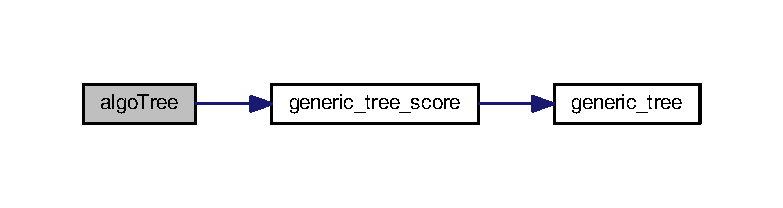
\includegraphics[width=350pt]{namespacealgo_ab46541a846c7f71c15e9bae5d5836af7_cgraph}
\end{center}
\end{figure}


\hypertarget{namespacealgo_a70c4b2737389dbfb07be3b39a8cf8e9b}{\index{algo@{algo}!find\-\_\-best\-\_\-k\-\_\-for\-\_\-kneighbors@{find\-\_\-best\-\_\-k\-\_\-for\-\_\-kneighbors}}
\index{find\-\_\-best\-\_\-k\-\_\-for\-\_\-kneighbors@{find\-\_\-best\-\_\-k\-\_\-for\-\_\-kneighbors}!algo@{algo}}
\subsubsection[{find\-\_\-best\-\_\-k\-\_\-for\-\_\-kneighbors}]{\setlength{\rightskip}{0pt plus 5cm}def algo.\-find\-\_\-best\-\_\-k\-\_\-for\-\_\-kneighbors (
\begin{DoxyParamCaption}
\item[{}]{X, }
\item[{}]{y, }
\item[{}]{n\-\_\-splits = {\ttfamily 5}, }
\item[{}]{show = {\ttfamily 0}}
\end{DoxyParamCaption}
)}}\label{namespacealgo_a70c4b2737389dbfb07be3b39a8cf8e9b}


permet de savoir le meilleur k possible 


\begin{DoxyParams}{Paramètres}
{\em X} & resultat de la tfidf \\
\hline
{\em y} & vecteur de la tfidf \\
\hline
{\em n\-\_\-splits,combien} & de sous ensemble pour la validation croisee \\
\hline
{\em show} & savoir si l'on dessine le graph \\
\hline
\end{DoxyParams}
\begin{DoxyReturn}{Renvoie}
best k 
\end{DoxyReturn}
\hypertarget{namespacealgo_a4227080ec2328a03c4f6f01e7b022e08}{\index{algo@{algo}!generic\-\_\-tree@{generic\-\_\-tree}}
\index{generic\-\_\-tree@{generic\-\_\-tree}!algo@{algo}}
\subsubsection[{generic\-\_\-tree}]{\setlength{\rightskip}{0pt plus 5cm}def algo.\-generic\-\_\-tree (
\begin{DoxyParamCaption}
\item[{}]{X, }
\item[{}]{y, }
\item[{}]{cls, }
\item[{}]{show = {\ttfamily 0}}
\end{DoxyParamCaption}
)}}\label{namespacealgo_a4227080ec2328a03c4f6f01e7b022e08}


permet de savoir les meilleurs parametres 


\begin{DoxyParams}{Paramètres}
{\em X} & resultat de la tfidf \\
\hline
{\em y} & vecteur de la tfidf \\
\hline
{\em cls} & fonction \\
\hline
{\em show} & savoir si l'on dessine le graph \\
\hline
\end{DoxyParams}
\begin{DoxyReturn}{Renvoie}
best\-\_\-min\-\_\-samples\-\_\-split,best\-\_\-max\-\_\-depth parametres optimaux 
\end{DoxyReturn}


Voici le graphe des appelants de cette fonction \-:
\nopagebreak
\begin{figure}[H]
\begin{center}
\leavevmode
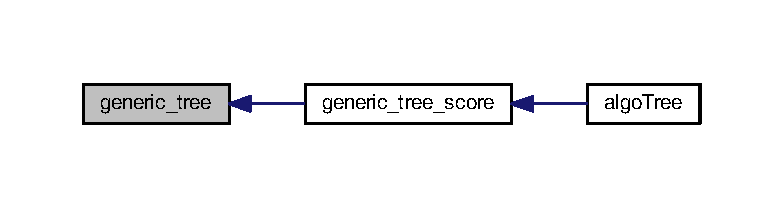
\includegraphics[width=350pt]{namespacealgo_a4227080ec2328a03c4f6f01e7b022e08_icgraph}
\end{center}
\end{figure}


\hypertarget{namespacealgo_a0afe8d007fc92279c75be5d0b40ecf07}{\index{algo@{algo}!generic\-\_\-tree\-\_\-score@{generic\-\_\-tree\-\_\-score}}
\index{generic\-\_\-tree\-\_\-score@{generic\-\_\-tree\-\_\-score}!algo@{algo}}
\subsubsection[{generic\-\_\-tree\-\_\-score}]{\setlength{\rightskip}{0pt plus 5cm}def algo.\-generic\-\_\-tree\-\_\-score (
\begin{DoxyParamCaption}
\item[{}]{X, }
\item[{}]{y, }
\item[{}]{matt, }
\item[{}]{vect, }
\item[{}]{cls, }
\item[{}]{show = {\ttfamily 0}}
\end{DoxyParamCaption}
)}}\label{namespacealgo_a0afe8d007fc92279c75be5d0b40ecf07}


permet de savoir si c'est un echec ou succes 


\begin{DoxyParams}{Paramètres}
{\em X} & resultat de la tfidf \\
\hline
{\em y} & vecteur de la tfidf \\
\hline
{\em matt} & resultat de la tfidf de test \\
\hline
{\em vect} & vecteur de la tfidf de test \\
\hline
{\em show} & savoir si l'on dessine le graph \\
\hline
\end{DoxyParams}
\begin{DoxyReturn}{Renvoie}
score en pourcentage 
\end{DoxyReturn}


Voici le graphe d'appel pour cette fonction \-:
\nopagebreak
\begin{figure}[H]
\begin{center}
\leavevmode
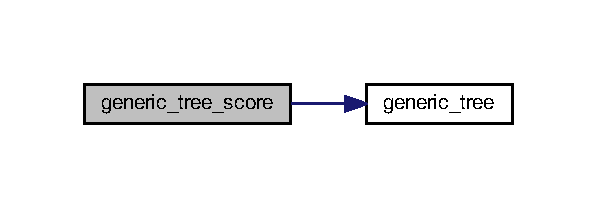
\includegraphics[width=286pt]{namespacealgo_a0afe8d007fc92279c75be5d0b40ecf07_cgraph}
\end{center}
\end{figure}




Voici le graphe des appelants de cette fonction \-:
\nopagebreak
\begin{figure}[H]
\begin{center}
\leavevmode
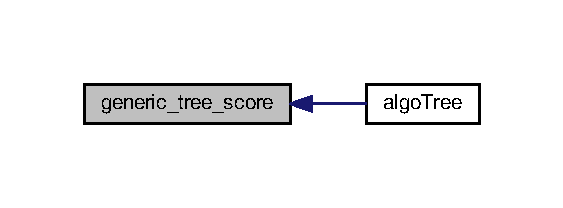
\includegraphics[width=270pt]{namespacealgo_a0afe8d007fc92279c75be5d0b40ecf07_icgraph}
\end{center}
\end{figure}


\hypertarget{namespacealgo_a5ecd48a13b42118beac0652265b8f353}{\index{algo@{algo}!naive\-Bayes@{naive\-Bayes}}
\index{naive\-Bayes@{naive\-Bayes}!algo@{algo}}
\subsubsection[{naive\-Bayes}]{\setlength{\rightskip}{0pt plus 5cm}def algo.\-naive\-Bayes (
\begin{DoxyParamCaption}
\item[{}]{mat, }
\item[{}]{vec, }
\item[{}]{matt, }
\item[{}]{vect}
\end{DoxyParamCaption}
)}}\label{namespacealgo_a5ecd48a13b42118beac0652265b8f353}


permet de savoir si c'est un echec ou succes 


\begin{DoxyParams}{Paramètres}
{\em mat} & resultat de la tfidf de train \\
\hline
{\em vec} & vecteur de la tfidf de train \\
\hline
{\em matt} & resultat de la tfidf de test \\
\hline
{\em vect} & vecteur de la tfidf de test \\
\hline
\end{DoxyParams}
\begin{DoxyReturn}{Renvoie}
score en pourcentage sur l'ensemble de test 
\end{DoxyReturn}
\hypertarget{namespacealgo_a9420060c614f9fb33cf05c91da71aee9}{\index{algo@{algo}!very\-Naive\-Bayes@{very\-Naive\-Bayes}}
\index{very\-Naive\-Bayes@{very\-Naive\-Bayes}!algo@{algo}}
\subsubsection[{very\-Naive\-Bayes}]{\setlength{\rightskip}{0pt plus 5cm}def algo.\-very\-Naive\-Bayes (
\begin{DoxyParamCaption}
\item[{}]{lt, }
\item[{}]{dic, }
\item[{}]{mat, }
\item[{}]{vec}
\end{DoxyParamCaption}
)}}\label{namespacealgo_a9420060c614f9fb33cf05c91da71aee9}


permet de savoir si c'est un echec ou succes 


\begin{DoxyParams}{Paramètres}
{\em lt} & list de tuples contenant (success, puis liste de mot) \\
\hline
{\em dic} & dictionnaire de la tfdif \\
\hline
{\em mat} & resultat de la tfidf \\
\hline
{\em vec} & vecteur de la tfidf \\
\hline
\end{DoxyParams}

\hypertarget{namespaceBDD}{\section{Référence de l'espace de nommage B\-D\-D}
\label{namespaceBDD}\index{B\-D\-D@{B\-D\-D}}
}
\subsection*{Classes}
\begin{DoxyCompactItemize}
\item 
class \hyperlink{classBDD_1_1BDD}{B\-D\-D}
\end{DoxyCompactItemize}
\subsection*{Variables}
\begin{DoxyCompactItemize}
\item 
string \hyperlink{namespaceBDD_a5b93a013f8d46f91f8d7b0fc102a42e7}{index} = \char`\"{}fouille\char`\"{}
\item 
string \hyperlink{namespaceBDD_ab065e06b98ff8f50dcdabe5715c5b710}{table\-Credit\-Test} = \char`\"{}Test\-Credit\char`\"{}
\item 
string \hyperlink{namespaceBDD_a5453a62b7989a6ea0d9d1f4016411323}{table\-Credit\-Train} = \char`\"{}Train\-Credit\char`\"{}
\item 
string \hyperlink{namespaceBDD_a1a3347461ee00b8dba8e995423d6acea}{table\-Movie\-Test} = \char`\"{}Test\-Movie\char`\"{}
\item 
string \hyperlink{namespaceBDD_a69bea8ff9373a0baf5bbf3df09f7a3b0}{table\-Movie\-Train} = \char`\"{}Train\-Movie\char`\"{}
\end{DoxyCompactItemize}


\subsection{Documentation des variables}
\hypertarget{namespaceBDD_a5b93a013f8d46f91f8d7b0fc102a42e7}{\index{B\-D\-D@{B\-D\-D}!index@{index}}
\index{index@{index}!BDD@{B\-D\-D}}
\subsubsection[{index}]{\setlength{\rightskip}{0pt plus 5cm}string index = \char`\"{}fouille\char`\"{}}}\label{namespaceBDD_a5b93a013f8d46f91f8d7b0fc102a42e7}
\hypertarget{namespaceBDD_ab065e06b98ff8f50dcdabe5715c5b710}{\index{B\-D\-D@{B\-D\-D}!table\-Credit\-Test@{table\-Credit\-Test}}
\index{table\-Credit\-Test@{table\-Credit\-Test}!BDD@{B\-D\-D}}
\subsubsection[{table\-Credit\-Test}]{\setlength{\rightskip}{0pt plus 5cm}string table\-Credit\-Test = \char`\"{}Test\-Credit\char`\"{}}}\label{namespaceBDD_ab065e06b98ff8f50dcdabe5715c5b710}
\hypertarget{namespaceBDD_a5453a62b7989a6ea0d9d1f4016411323}{\index{B\-D\-D@{B\-D\-D}!table\-Credit\-Train@{table\-Credit\-Train}}
\index{table\-Credit\-Train@{table\-Credit\-Train}!BDD@{B\-D\-D}}
\subsubsection[{table\-Credit\-Train}]{\setlength{\rightskip}{0pt plus 5cm}string table\-Credit\-Train = \char`\"{}Train\-Credit\char`\"{}}}\label{namespaceBDD_a5453a62b7989a6ea0d9d1f4016411323}
\hypertarget{namespaceBDD_a1a3347461ee00b8dba8e995423d6acea}{\index{B\-D\-D@{B\-D\-D}!table\-Movie\-Test@{table\-Movie\-Test}}
\index{table\-Movie\-Test@{table\-Movie\-Test}!BDD@{B\-D\-D}}
\subsubsection[{table\-Movie\-Test}]{\setlength{\rightskip}{0pt plus 5cm}string table\-Movie\-Test = \char`\"{}Test\-Movie\char`\"{}}}\label{namespaceBDD_a1a3347461ee00b8dba8e995423d6acea}
\hypertarget{namespaceBDD_a69bea8ff9373a0baf5bbf3df09f7a3b0}{\index{B\-D\-D@{B\-D\-D}!table\-Movie\-Train@{table\-Movie\-Train}}
\index{table\-Movie\-Train@{table\-Movie\-Train}!BDD@{B\-D\-D}}
\subsubsection[{table\-Movie\-Train}]{\setlength{\rightskip}{0pt plus 5cm}string table\-Movie\-Train = \char`\"{}Train\-Movie\char`\"{}}}\label{namespaceBDD_a69bea8ff9373a0baf5bbf3df09f7a3b0}

\hypertarget{namespacemain}{\section{Référence de l'espace de nommage main}
\label{namespacemain}\index{main@{main}}
}
\subsection*{Variables}
\begin{DoxyCompactItemize}
\item 
tuple \hyperlink{namespacemain_a3ba02571b750dd172f300851ef10228e}{dic} = to.\-get\-Dict(tfidf)
\item 
tuple \hyperlink{namespacemain_abc599b1f87ca3a4e0ff709091fb25176}{l} = to.\-create\-List(d, s)
\item 
tuple \hyperlink{namespacemain_a2187ed276d33f5f18ef29ecf5ce613ba}{lt} = to.\-create\-List(dt, st)
\item 
tuple \hyperlink{namespacemain_a7a74e6f2f6355f34b63513f77c839a9e}{x} = al.\-find\-\_\-best\-\_\-k\-\_\-for\-\_\-kneighbors(mat, vec)
\end{DoxyCompactItemize}


\subsection{Documentation des variables}
\hypertarget{namespacemain_a3ba02571b750dd172f300851ef10228e}{\index{main@{main}!dic@{dic}}
\index{dic@{dic}!main@{main}}
\subsubsection[{dic}]{\setlength{\rightskip}{0pt plus 5cm}tuple dic = to.\-get\-Dict(tfidf)}}\label{namespacemain_a3ba02571b750dd172f300851ef10228e}
\hypertarget{namespacemain_abc599b1f87ca3a4e0ff709091fb25176}{\index{main@{main}!l@{l}}
\index{l@{l}!main@{main}}
\subsubsection[{l}]{\setlength{\rightskip}{0pt plus 5cm}tuple l = to.\-create\-List(d, s)}}\label{namespacemain_abc599b1f87ca3a4e0ff709091fb25176}
\hypertarget{namespacemain_a2187ed276d33f5f18ef29ecf5ce613ba}{\index{main@{main}!lt@{lt}}
\index{lt@{lt}!main@{main}}
\subsubsection[{lt}]{\setlength{\rightskip}{0pt plus 5cm}tuple lt = to.\-create\-List(dt, st)}}\label{namespacemain_a2187ed276d33f5f18ef29ecf5ce613ba}
\hypertarget{namespacemain_a7a74e6f2f6355f34b63513f77c839a9e}{\index{main@{main}!x@{x}}
\index{x@{x}!main@{main}}
\subsubsection[{x}]{\setlength{\rightskip}{0pt plus 5cm}tuple x = al.\-find\-\_\-best\-\_\-k\-\_\-for\-\_\-kneighbors(mat, vec)}}\label{namespacemain_a7a74e6f2f6355f34b63513f77c839a9e}

\hypertarget{namespaceoperatorBDD}{\section{Référence de l'espace de nommage operator\-B\-D\-D}
\label{namespaceoperatorBDD}\index{operator\-B\-D\-D@{operator\-B\-D\-D}}
}
\subsection*{Fonctions}
\begin{DoxyCompactItemize}
\item 
def \hyperlink{namespaceoperatorBDD_a5aaccf3717ce1479bbd6ef2a0ffcbf49}{B\-D\-Dfrom\-C\-S\-V}
\begin{DoxyCompactList}\small\item\em permet de stocker dans elasticsearch les donnees dans fichiers \end{DoxyCompactList}\item 
def \hyperlink{namespaceoperatorBDD_a9890bc0308c65dae331300c93f804b11}{B\-D\-D\-Search}
\begin{DoxyCompactList}\small\item\em cherche dans la table, la requete et renvoi le resultat \end{DoxyCompactList}\item 
def \hyperlink{namespaceoperatorBDD_a84ebaeadd8b021780f5fa72f73bf3ea3}{B\-D\-D\-Search\-All}
\begin{DoxyCompactList}\small\item\em cherche dans la table train, tout les documents \end{DoxyCompactList}\item 
def \hyperlink{namespaceoperatorBDD_aa9ab222b23d1b7a6e094fb82d702cd0a}{B\-D\-D\-Search\-All\-Test}
\begin{DoxyCompactList}\small\item\em cherche dans la table test, tout les documents \end{DoxyCompactList}\item 
def \hyperlink{namespaceoperatorBDD_a03889cf9d5fd998892c621491a12142b}{B\-D\-D\-Search\-Categorie}
\begin{DoxyCompactList}\small\item\em cherche dans la table train, tout les documents ayant tel key et value \end{DoxyCompactList}\item 
def \hyperlink{namespaceoperatorBDD_a30969a6c243559357c836ae43365877b}{B\-D\-D\-Search\-Categorie\-Test}
\begin{DoxyCompactList}\small\item\em cherche dans la table test, tout les documents ayant tel key et value \end{DoxyCompactList}\end{DoxyCompactItemize}
\subsection*{Variables}
\begin{DoxyCompactItemize}
\item 
float \hyperlink{namespaceoperatorBDD_a131e5e7a22125521cf2cb5eb732a0f54}{mediane\-Vote\-Average} = 6.\-2
\end{DoxyCompactItemize}


\subsection{Documentation des fonctions}
\hypertarget{namespaceoperatorBDD_a5aaccf3717ce1479bbd6ef2a0ffcbf49}{\index{operator\-B\-D\-D@{operator\-B\-D\-D}!B\-D\-Dfrom\-C\-S\-V@{B\-D\-Dfrom\-C\-S\-V}}
\index{B\-D\-Dfrom\-C\-S\-V@{B\-D\-Dfrom\-C\-S\-V}!operatorBDD@{operator\-B\-D\-D}}
\subsubsection[{B\-D\-Dfrom\-C\-S\-V}]{\setlength{\rightskip}{0pt plus 5cm}def operator\-B\-D\-D.\-B\-D\-Dfrom\-C\-S\-V (
\begin{DoxyParamCaption}
\item[{}]{csv\-\_\-filename\-Movie, }
\item[{}]{csv\-\_\-filename\-Credit, }
\item[{}]{table\-Train, }
\item[{}]{table\-Test, }
\item[{}]{number\-Separation}
\end{DoxyParamCaption}
)}}\label{namespaceoperatorBDD_a5aaccf3717ce1479bbd6ef2a0ffcbf49}


permet de stocker dans elasticsearch les donnees dans fichiers 


\begin{DoxyParams}{Paramètres}
{\em csv\-\_\-filename\-Movie} & chemin du fichier des films \\
\hline
{\em csv\-\_\-filename\-Credit} & chemin du fichier des credits \\
\hline
{\em table\-Train} & name table d'entrainement \\
\hline
{\em table\-Test} & name table de test \\
\hline
{\em number\-Separation} & nombre ou la separation a lieu entre les deux tables \\
\hline
\end{DoxyParams}
\hypertarget{namespaceoperatorBDD_a9890bc0308c65dae331300c93f804b11}{\index{operator\-B\-D\-D@{operator\-B\-D\-D}!B\-D\-D\-Search@{B\-D\-D\-Search}}
\index{B\-D\-D\-Search@{B\-D\-D\-Search}!operatorBDD@{operator\-B\-D\-D}}
\subsubsection[{B\-D\-D\-Search}]{\setlength{\rightskip}{0pt plus 5cm}def operator\-B\-D\-D.\-B\-D\-D\-Search (
\begin{DoxyParamCaption}
\item[{}]{query, }
\item[{}]{table}
\end{DoxyParamCaption}
)}}\label{namespaceoperatorBDD_a9890bc0308c65dae331300c93f804b11}


cherche dans la table, la requete et renvoi le resultat 


\begin{DoxyParams}{Paramètres}
{\em query} & requete a faire dnas la base \\
\hline
{\em table} & sur quel table effectue la requete \\
\hline
\end{DoxyParams}
\begin{DoxyReturn}{Renvoie}
resultat de la requete 
\end{DoxyReturn}


Voici le graphe des appelants de cette fonction \-:
\nopagebreak
\begin{figure}[H]
\begin{center}
\leavevmode
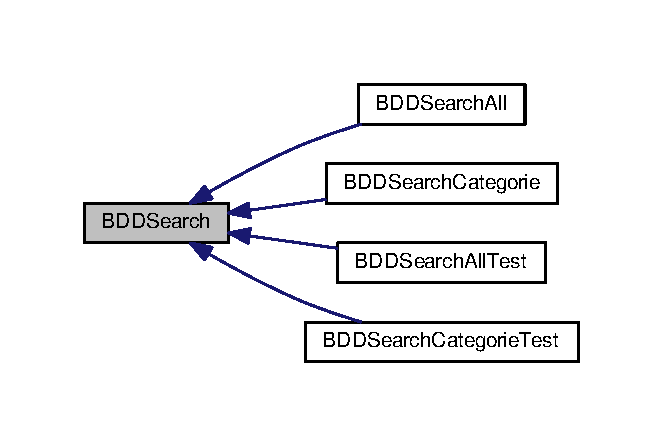
\includegraphics[width=318pt]{namespaceoperatorBDD_a9890bc0308c65dae331300c93f804b11_icgraph}
\end{center}
\end{figure}


\hypertarget{namespaceoperatorBDD_a84ebaeadd8b021780f5fa72f73bf3ea3}{\index{operator\-B\-D\-D@{operator\-B\-D\-D}!B\-D\-D\-Search\-All@{B\-D\-D\-Search\-All}}
\index{B\-D\-D\-Search\-All@{B\-D\-D\-Search\-All}!operatorBDD@{operator\-B\-D\-D}}
\subsubsection[{B\-D\-D\-Search\-All}]{\setlength{\rightskip}{0pt plus 5cm}def operator\-B\-D\-D.\-B\-D\-D\-Search\-All (
\begin{DoxyParamCaption}
{}
\end{DoxyParamCaption}
)}}\label{namespaceoperatorBDD_a84ebaeadd8b021780f5fa72f73bf3ea3}


cherche dans la table train, tout les documents 

\begin{DoxyReturn}{Renvoie}
resultat de la requete 
\end{DoxyReturn}


Voici le graphe d'appel pour cette fonction \-:
\nopagebreak
\begin{figure}[H]
\begin{center}
\leavevmode
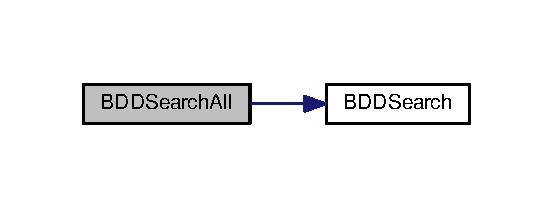
\includegraphics[width=266pt]{namespaceoperatorBDD_a84ebaeadd8b021780f5fa72f73bf3ea3_cgraph}
\end{center}
\end{figure}


\hypertarget{namespaceoperatorBDD_aa9ab222b23d1b7a6e094fb82d702cd0a}{\index{operator\-B\-D\-D@{operator\-B\-D\-D}!B\-D\-D\-Search\-All\-Test@{B\-D\-D\-Search\-All\-Test}}
\index{B\-D\-D\-Search\-All\-Test@{B\-D\-D\-Search\-All\-Test}!operatorBDD@{operator\-B\-D\-D}}
\subsubsection[{B\-D\-D\-Search\-All\-Test}]{\setlength{\rightskip}{0pt plus 5cm}def operator\-B\-D\-D.\-B\-D\-D\-Search\-All\-Test (
\begin{DoxyParamCaption}
{}
\end{DoxyParamCaption}
)}}\label{namespaceoperatorBDD_aa9ab222b23d1b7a6e094fb82d702cd0a}


cherche dans la table test, tout les documents 

\begin{DoxyReturn}{Renvoie}
resultat de la requete 
\end{DoxyReturn}


Voici le graphe d'appel pour cette fonction \-:
\nopagebreak
\begin{figure}[H]
\begin{center}
\leavevmode
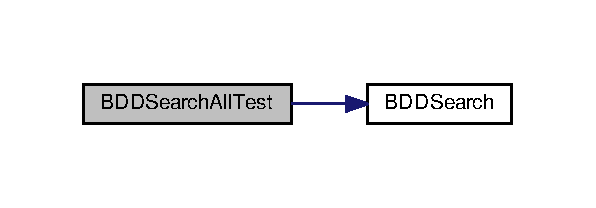
\includegraphics[width=286pt]{namespaceoperatorBDD_aa9ab222b23d1b7a6e094fb82d702cd0a_cgraph}
\end{center}
\end{figure}


\hypertarget{namespaceoperatorBDD_a03889cf9d5fd998892c621491a12142b}{\index{operator\-B\-D\-D@{operator\-B\-D\-D}!B\-D\-D\-Search\-Categorie@{B\-D\-D\-Search\-Categorie}}
\index{B\-D\-D\-Search\-Categorie@{B\-D\-D\-Search\-Categorie}!operatorBDD@{operator\-B\-D\-D}}
\subsubsection[{B\-D\-D\-Search\-Categorie}]{\setlength{\rightskip}{0pt plus 5cm}def operator\-B\-D\-D.\-B\-D\-D\-Search\-Categorie (
\begin{DoxyParamCaption}
\item[{}]{key, }
\item[{}]{value}
\end{DoxyParamCaption}
)}}\label{namespaceoperatorBDD_a03889cf9d5fd998892c621491a12142b}


cherche dans la table train, tout les documents ayant tel key et value 


\begin{DoxyParams}{Paramètres}
{\em key} & le champs sur lequel faire une requete \\
\hline
{\em value} & la valeur du champs \\
\hline
\end{DoxyParams}
\begin{DoxyReturn}{Renvoie}
resultat de la requete 
\end{DoxyReturn}


Voici le graphe d'appel pour cette fonction \-:
\nopagebreak
\begin{figure}[H]
\begin{center}
\leavevmode
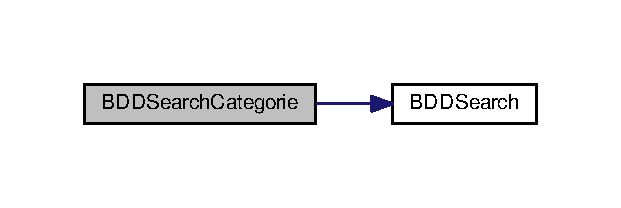
\includegraphics[width=298pt]{namespaceoperatorBDD_a03889cf9d5fd998892c621491a12142b_cgraph}
\end{center}
\end{figure}


\hypertarget{namespaceoperatorBDD_a30969a6c243559357c836ae43365877b}{\index{operator\-B\-D\-D@{operator\-B\-D\-D}!B\-D\-D\-Search\-Categorie\-Test@{B\-D\-D\-Search\-Categorie\-Test}}
\index{B\-D\-D\-Search\-Categorie\-Test@{B\-D\-D\-Search\-Categorie\-Test}!operatorBDD@{operator\-B\-D\-D}}
\subsubsection[{B\-D\-D\-Search\-Categorie\-Test}]{\setlength{\rightskip}{0pt plus 5cm}def operator\-B\-D\-D.\-B\-D\-D\-Search\-Categorie\-Test (
\begin{DoxyParamCaption}
\item[{}]{key, }
\item[{}]{value}
\end{DoxyParamCaption}
)}}\label{namespaceoperatorBDD_a30969a6c243559357c836ae43365877b}


cherche dans la table test, tout les documents ayant tel key et value 


\begin{DoxyParams}{Paramètres}
{\em key} & le champs sur lequel faire une requete \\
\hline
{\em value} & la valeur du champs \\
\hline
\end{DoxyParams}
\begin{DoxyReturn}{Renvoie}
resultat de la requete 
\end{DoxyReturn}


Voici le graphe d'appel pour cette fonction \-:
\nopagebreak
\begin{figure}[H]
\begin{center}
\leavevmode
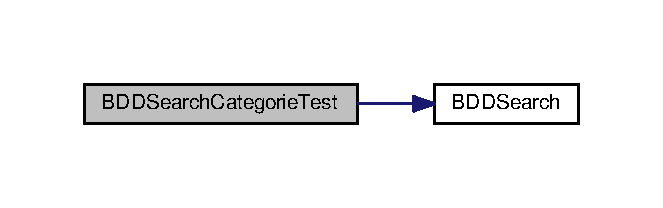
\includegraphics[width=318pt]{namespaceoperatorBDD_a30969a6c243559357c836ae43365877b_cgraph}
\end{center}
\end{figure}




\subsection{Documentation des variables}
\hypertarget{namespaceoperatorBDD_a131e5e7a22125521cf2cb5eb732a0f54}{\index{operator\-B\-D\-D@{operator\-B\-D\-D}!mediane\-Vote\-Average@{mediane\-Vote\-Average}}
\index{mediane\-Vote\-Average@{mediane\-Vote\-Average}!operatorBDD@{operator\-B\-D\-D}}
\subsubsection[{mediane\-Vote\-Average}]{\setlength{\rightskip}{0pt plus 5cm}float mediane\-Vote\-Average = 6.\-2}}\label{namespaceoperatorBDD_a131e5e7a22125521cf2cb5eb732a0f54}

\hypertarget{namespacetoolsBDD}{\section{Référence de l'espace de nommage tools\-B\-D\-D}
\label{namespacetoolsBDD}\index{tools\-B\-D\-D@{tools\-B\-D\-D}}
}
\subsection*{Fonctions}
\begin{DoxyCompactItemize}
\item 
def \hyperlink{namespacetoolsBDD_abf21310dd3cdd39ff5f781eaafb23b24}{concat\-Data}
\begin{DoxyCompactList}\small\item\em permet de concatener les valeurs \end{DoxyCompactList}\item 
def \hyperlink{namespacetoolsBDD_afc4367a1a711e612f8f4d6363edbc640}{create\-List}
\begin{DoxyCompactList}\small\item\em liste of tuple \end{DoxyCompactList}\item 
def \hyperlink{namespacetoolsBDD_a60efb6c205d51bf9a9e32b6d19f633b4}{get\-\_\-train\-\_\-test\-\_\-sets}
\begin{DoxyCompactList}\small\item\em permet de creer faire des separation pour la validation croisee \end{DoxyCompactList}\item 
def \hyperlink{namespacetoolsBDD_ae897b96e0c4a89d09f418e620819a066}{get\-All\-\_\-\-Vote\-Average}
\begin{DoxyCompactList}\small\item\em recuperer tous les votes \end{DoxyCompactList}\item 
def \hyperlink{namespacetoolsBDD_a15b2ef52eec23442bb79863d794e2e2b}{get\-Cast}
\begin{DoxyCompactList}\small\item\em permet de contaner les valeurs des 6 acteurs dans une chaine de char \end{DoxyCompactList}\item 
def \hyperlink{namespacetoolsBDD_ab6a097315bef68f12966b652fd120913}{get\-Data}
\begin{DoxyCompactList}\small\item\em permet de contaner les valeurs dans une chaine de char \end{DoxyCompactList}\item 
def \hyperlink{namespacetoolsBDD_a1815eb69cbba2e6abc16b649baa2fdad}{get\-Data\-\_\-\-Vote\-Average}
\begin{DoxyCompactList}\small\item\em calcul des statistiques sur le champ vote\-\_\-average \end{DoxyCompactList}\item 
def \hyperlink{namespacetoolsBDD_aef96b5903d59864e793f4377d82bac25}{get\-Dict}
\begin{DoxyCompactList}\small\item\em permet de connaitre les labels dune tfidf \end{DoxyCompactList}\item 
def \hyperlink{namespacetoolsBDD_abc6b8127dc8f28edc53d719a4835bfa3}{get\-Essential\-Test}
\begin{DoxyCompactList}\small\item\em permet de recuperer les infos pour ensemble de train \end{DoxyCompactList}\item 
def \hyperlink{namespacetoolsBDD_ab85cfda40b715e400dda4a5e5c97f9ce}{get\-Essential\-Train}
\begin{DoxyCompactList}\small\item\em permet de recuperer les infos pour ensemble de train \end{DoxyCompactList}\item 
def \hyperlink{namespacetoolsBDD_ad9d092a50decbd07a5130e144731caa9}{get\-Real}
\begin{DoxyCompactList}\small\item\em permet de contaner les realisateurs dans une chaine de char \end{DoxyCompactList}\item 
def \hyperlink{namespacetoolsBDD_ae224e914a0d4d23030401af6e59cb1bc}{get\-Size}
\begin{DoxyCompactList}\small\item\em permet de savoir le nombre de hits \end{DoxyCompactList}\item 
def \hyperlink{namespacetoolsBDD_a49928e1495cbb0687a8656f3c5481d5b}{get\-Test}
\begin{DoxyCompactList}\small\item\em return an index for tfidf, None if doesn't exist \end{DoxyCompactList}\item 
def \hyperlink{namespacetoolsBDD_ae5e38adc6d6db8e1ece60d2bc307a39f}{init}
\begin{DoxyCompactList}\small\item\em permet de charger dans la base de donnee \end{DoxyCompactList}\item 
def \hyperlink{namespacetoolsBDD_a82b711337498f7fa58e3c9d784415424}{ranking}
\begin{DoxyCompactList}\small\item\em calcul le nombre de film dont le score $>$= x \end{DoxyCompactList}\item 
def \hyperlink{namespacetoolsBDD_a2e502b4dae284eb951de46e92134895f}{stat}
\begin{DoxyCompactList}\small\item\em permet de calculer et d'afficher des statistiques \end{DoxyCompactList}\item 
def \hyperlink{namespacetoolsBDD_a73bb9d4526a9cd6825636ef1a5777106}{test\-\_\-success}
\begin{DoxyCompactList}\small\item\em permet de savoir si cela est un succes \end{DoxyCompactList}\item 
def \hyperlink{namespacetoolsBDD_a07b4809d77a061cf4c10d05b35edf657}{test\-\_\-success2}
\begin{DoxyCompactList}\small\item\em permet de savoir si cela est un succes \end{DoxyCompactList}\item 
def \hyperlink{namespacetoolsBDD_accbe8232ffba571517272bcd0eb22df7}{transform}
\begin{DoxyCompactList}\small\item\em permet d'effectuer un tfidf \end{DoxyCompactList}\end{DoxyCompactItemize}


\subsection{Documentation des fonctions}
\hypertarget{namespacetoolsBDD_abf21310dd3cdd39ff5f781eaafb23b24}{\index{tools\-B\-D\-D@{tools\-B\-D\-D}!concat\-Data@{concat\-Data}}
\index{concat\-Data@{concat\-Data}!toolsBDD@{tools\-B\-D\-D}}
\subsubsection[{concat\-Data}]{\setlength{\rightskip}{0pt plus 5cm}def tools\-B\-D\-D.\-concat\-Data (
\begin{DoxyParamCaption}
\item[{}]{d, }
\item[{}]{si, }
\item[{}]{i}
\end{DoxyParamCaption}
)}}\label{namespacetoolsBDD_abf21310dd3cdd39ff5f781eaafb23b24}


permet de concatener les valeurs 


\begin{DoxyParams}{Paramètres}
{\em d} & toutes les lignes \\
\hline
{\em si} & nombre de lignes \\
\hline
{\em i} & le numero de la ligne courante \\
\hline
\end{DoxyParams}
\begin{DoxyReturn}{Renvoie}
char$\ast$ 
\end{DoxyReturn}


Voici le graphe d'appel pour cette fonction \-:\nopagebreak
\begin{figure}[H]
\begin{center}
\leavevmode
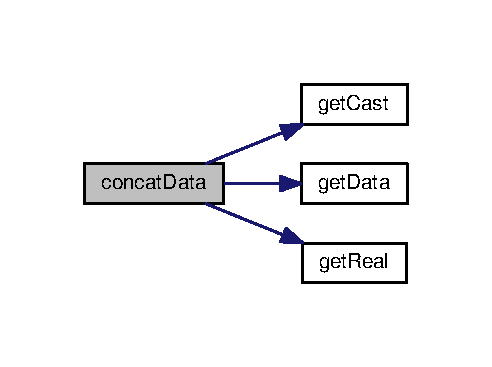
\includegraphics[width=236pt]{namespacetoolsBDD_abf21310dd3cdd39ff5f781eaafb23b24_cgraph}
\end{center}
\end{figure}




Voici le graphe des appelants de cette fonction \-:\nopagebreak
\begin{figure}[H]
\begin{center}
\leavevmode
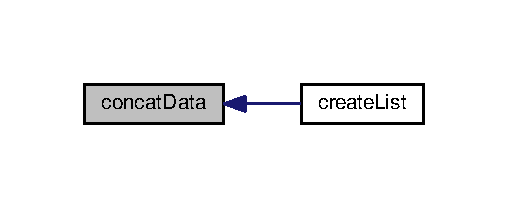
\includegraphics[width=244pt]{namespacetoolsBDD_abf21310dd3cdd39ff5f781eaafb23b24_icgraph}
\end{center}
\end{figure}


\hypertarget{namespacetoolsBDD_afc4367a1a711e612f8f4d6363edbc640}{\index{tools\-B\-D\-D@{tools\-B\-D\-D}!create\-List@{create\-List}}
\index{create\-List@{create\-List}!toolsBDD@{tools\-B\-D\-D}}
\subsubsection[{create\-List}]{\setlength{\rightskip}{0pt plus 5cm}def tools\-B\-D\-D.\-create\-List (
\begin{DoxyParamCaption}
\item[{}]{d, }
\item[{}]{si}
\end{DoxyParamCaption}
)}}\label{namespacetoolsBDD_afc4367a1a711e612f8f4d6363edbc640}


liste of tuple 


\begin{DoxyParams}{Paramètres}
{\em d} & toutes les lignes \\
\hline
{\em si} & nombre de lignes \\
\hline
\end{DoxyParams}
\begin{DoxyReturn}{Renvoie}
list of tuple 
\end{DoxyReturn}


Voici le graphe d'appel pour cette fonction \-:\nopagebreak
\begin{figure}[H]
\begin{center}
\leavevmode
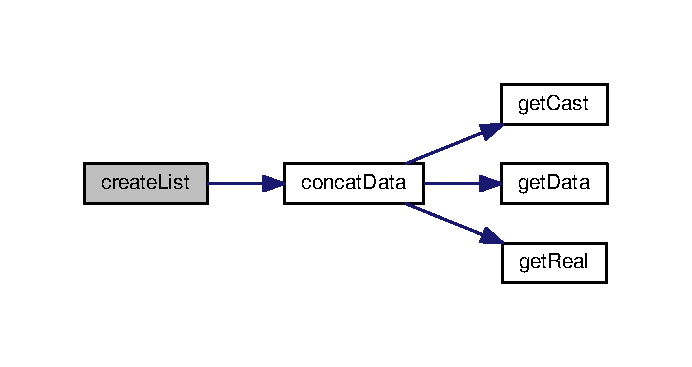
\includegraphics[width=332pt]{namespacetoolsBDD_afc4367a1a711e612f8f4d6363edbc640_cgraph}
\end{center}
\end{figure}


\hypertarget{namespacetoolsBDD_a60efb6c205d51bf9a9e32b6d19f633b4}{\index{tools\-B\-D\-D@{tools\-B\-D\-D}!get\-\_\-train\-\_\-test\-\_\-sets@{get\-\_\-train\-\_\-test\-\_\-sets}}
\index{get\-\_\-train\-\_\-test\-\_\-sets@{get\-\_\-train\-\_\-test\-\_\-sets}!toolsBDD@{tools\-B\-D\-D}}
\subsubsection[{get\-\_\-train\-\_\-test\-\_\-sets}]{\setlength{\rightskip}{0pt plus 5cm}def tools\-B\-D\-D.\-get\-\_\-train\-\_\-test\-\_\-sets (
\begin{DoxyParamCaption}
\item[{}]{X, }
\item[{}]{y}
\end{DoxyParamCaption}
)}}\label{namespacetoolsBDD_a60efb6c205d51bf9a9e32b6d19f633b4}


permet de creer faire des separation pour la validation croisee 


\begin{DoxyParams}{Paramètres}
{\em X} & resultat de la tfidf \\
\hline
{\em y} & vecteur de la tfidf \\
\hline
\end{DoxyParams}
\begin{DoxyReturn}{Renvoie}
split 
\end{DoxyReturn}
\hypertarget{namespacetoolsBDD_ae897b96e0c4a89d09f418e620819a066}{\index{tools\-B\-D\-D@{tools\-B\-D\-D}!get\-All\-\_\-\-Vote\-Average@{get\-All\-\_\-\-Vote\-Average}}
\index{get\-All\-\_\-\-Vote\-Average@{get\-All\-\_\-\-Vote\-Average}!toolsBDD@{tools\-B\-D\-D}}
\subsubsection[{get\-All\-\_\-\-Vote\-Average}]{\setlength{\rightskip}{0pt plus 5cm}def tools\-B\-D\-D.\-get\-All\-\_\-\-Vote\-Average (
\begin{DoxyParamCaption}
\item[{}]{d, }
\item[{}]{si}
\end{DoxyParamCaption}
)}}\label{namespacetoolsBDD_ae897b96e0c4a89d09f418e620819a066}


recuperer tous les votes 


\begin{DoxyParams}{Paramètres}
{\em d} & toutes les lignes \\
\hline
{\em si} & nombre de lignes \\
\hline
\end{DoxyParams}
\begin{DoxyReturn}{Renvoie}
a numpy array \-: list 
\end{DoxyReturn}


Voici le graphe des appelants de cette fonction \-:\nopagebreak
\begin{figure}[H]
\begin{center}
\leavevmode
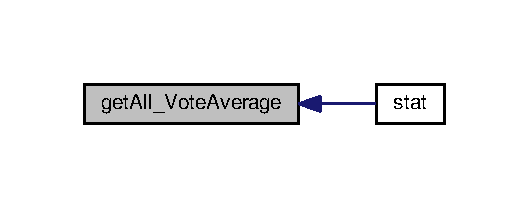
\includegraphics[width=254pt]{namespacetoolsBDD_ae897b96e0c4a89d09f418e620819a066_icgraph}
\end{center}
\end{figure}


\hypertarget{namespacetoolsBDD_a15b2ef52eec23442bb79863d794e2e2b}{\index{tools\-B\-D\-D@{tools\-B\-D\-D}!get\-Cast@{get\-Cast}}
\index{get\-Cast@{get\-Cast}!toolsBDD@{tools\-B\-D\-D}}
\subsubsection[{get\-Cast}]{\setlength{\rightskip}{0pt plus 5cm}def tools\-B\-D\-D.\-get\-Cast (
\begin{DoxyParamCaption}
\item[{}]{d, }
\item[{}]{si, }
\item[{}]{a}
\end{DoxyParamCaption}
)}}\label{namespacetoolsBDD_a15b2ef52eec23442bb79863d794e2e2b}


permet de contaner les valeurs des 6 acteurs dans une chaine de char 


\begin{DoxyParams}{Paramètres}
{\em d} & toutes les lignes \\
\hline
{\em si} & nombre de lignes \\
\hline
{\em a} & le numero de la ligne courante \\
\hline
\end{DoxyParams}
\begin{DoxyReturn}{Renvoie}
char$\ast$ 
\end{DoxyReturn}


Voici le graphe des appelants de cette fonction \-:\nopagebreak
\begin{figure}[H]
\begin{center}
\leavevmode
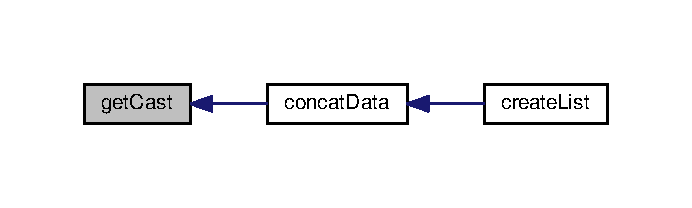
\includegraphics[width=332pt]{namespacetoolsBDD_a15b2ef52eec23442bb79863d794e2e2b_icgraph}
\end{center}
\end{figure}


\hypertarget{namespacetoolsBDD_ab6a097315bef68f12966b652fd120913}{\index{tools\-B\-D\-D@{tools\-B\-D\-D}!get\-Data@{get\-Data}}
\index{get\-Data@{get\-Data}!toolsBDD@{tools\-B\-D\-D}}
\subsubsection[{get\-Data}]{\setlength{\rightskip}{0pt plus 5cm}def tools\-B\-D\-D.\-get\-Data (
\begin{DoxyParamCaption}
\item[{}]{d, }
\item[{}]{si, }
\item[{}]{a, }
\item[{}]{typ}
\end{DoxyParamCaption}
)}}\label{namespacetoolsBDD_ab6a097315bef68f12966b652fd120913}


permet de contaner les valeurs dans une chaine de char 


\begin{DoxyParams}{Paramètres}
{\em d} & toutes les lignes \\
\hline
{\em si} & nombre de lignes \\
\hline
{\em a} & le numero de la ligne courante \\
\hline
{\em typ} & le champs a regarder \\
\hline
\end{DoxyParams}
\begin{DoxyReturn}{Renvoie}
char$\ast$ 
\end{DoxyReturn}


Voici le graphe des appelants de cette fonction \-:\nopagebreak
\begin{figure}[H]
\begin{center}
\leavevmode
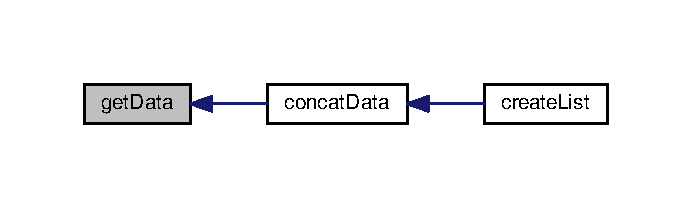
\includegraphics[width=332pt]{namespacetoolsBDD_ab6a097315bef68f12966b652fd120913_icgraph}
\end{center}
\end{figure}


\hypertarget{namespacetoolsBDD_a1815eb69cbba2e6abc16b649baa2fdad}{\index{tools\-B\-D\-D@{tools\-B\-D\-D}!get\-Data\-\_\-\-Vote\-Average@{get\-Data\-\_\-\-Vote\-Average}}
\index{get\-Data\-\_\-\-Vote\-Average@{get\-Data\-\_\-\-Vote\-Average}!toolsBDD@{tools\-B\-D\-D}}
\subsubsection[{get\-Data\-\_\-\-Vote\-Average}]{\setlength{\rightskip}{0pt plus 5cm}def tools\-B\-D\-D.\-get\-Data\-\_\-\-Vote\-Average (
\begin{DoxyParamCaption}
\item[{}]{t}
\end{DoxyParamCaption}
)}}\label{namespacetoolsBDD_a1815eb69cbba2e6abc16b649baa2fdad}


calcul des statistiques sur le champ vote\-\_\-average 


\begin{DoxyParams}{Paramètres}
{\em t} & une ligne \\
\hline
\end{DoxyParams}
\begin{DoxyReturn}{Renvoie}
moyenne, median, variance, ecart de vote\-\_\-average 
\end{DoxyReturn}


Voici le graphe des appelants de cette fonction \-:\nopagebreak
\begin{figure}[H]
\begin{center}
\leavevmode
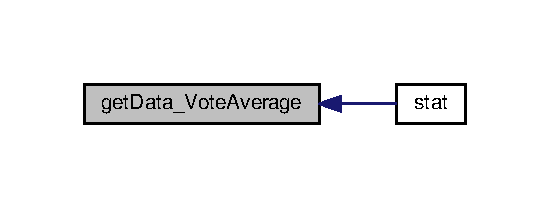
\includegraphics[width=264pt]{namespacetoolsBDD_a1815eb69cbba2e6abc16b649baa2fdad_icgraph}
\end{center}
\end{figure}


\hypertarget{namespacetoolsBDD_aef96b5903d59864e793f4377d82bac25}{\index{tools\-B\-D\-D@{tools\-B\-D\-D}!get\-Dict@{get\-Dict}}
\index{get\-Dict@{get\-Dict}!toolsBDD@{tools\-B\-D\-D}}
\subsubsection[{get\-Dict}]{\setlength{\rightskip}{0pt plus 5cm}def tools\-B\-D\-D.\-get\-Dict (
\begin{DoxyParamCaption}
\item[{}]{tfidf}
\end{DoxyParamCaption}
)}}\label{namespacetoolsBDD_aef96b5903d59864e793f4377d82bac25}


permet de connaitre les labels dune tfidf 


\begin{DoxyParams}{Paramètres}
{\em tfidf} & ou recuperer le vocabulaire \\
\hline
\end{DoxyParams}
\begin{DoxyReturn}{Renvoie}
le vocabulaire de la tf-\/idf 
\end{DoxyReturn}
\hypertarget{namespacetoolsBDD_abc6b8127dc8f28edc53d719a4835bfa3}{\index{tools\-B\-D\-D@{tools\-B\-D\-D}!get\-Essential\-Test@{get\-Essential\-Test}}
\index{get\-Essential\-Test@{get\-Essential\-Test}!toolsBDD@{tools\-B\-D\-D}}
\subsubsection[{get\-Essential\-Test}]{\setlength{\rightskip}{0pt plus 5cm}def tools\-B\-D\-D.\-get\-Essential\-Test (
\begin{DoxyParamCaption}
{}
\end{DoxyParamCaption}
)}}\label{namespacetoolsBDD_abc6b8127dc8f28edc53d719a4835bfa3}


permet de recuperer les infos pour ensemble de train 

\begin{DoxyReturn}{Renvoie}
a,s,d les lignes de la base, le nombre et un dict 
\end{DoxyReturn}


Voici le graphe d'appel pour cette fonction \-:\nopagebreak
\begin{figure}[H]
\begin{center}
\leavevmode
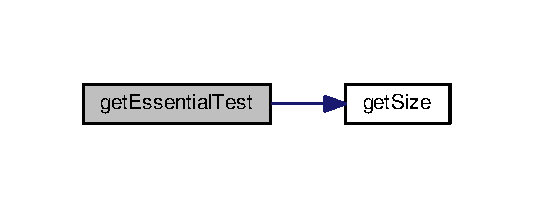
\includegraphics[width=256pt]{namespacetoolsBDD_abc6b8127dc8f28edc53d719a4835bfa3_cgraph}
\end{center}
\end{figure}


\hypertarget{namespacetoolsBDD_ab85cfda40b715e400dda4a5e5c97f9ce}{\index{tools\-B\-D\-D@{tools\-B\-D\-D}!get\-Essential\-Train@{get\-Essential\-Train}}
\index{get\-Essential\-Train@{get\-Essential\-Train}!toolsBDD@{tools\-B\-D\-D}}
\subsubsection[{get\-Essential\-Train}]{\setlength{\rightskip}{0pt plus 5cm}def tools\-B\-D\-D.\-get\-Essential\-Train (
\begin{DoxyParamCaption}
{}
\end{DoxyParamCaption}
)}}\label{namespacetoolsBDD_ab85cfda40b715e400dda4a5e5c97f9ce}


permet de recuperer les infos pour ensemble de train 

\begin{DoxyReturn}{Renvoie}
a,s,d les lignes de la base, le nombre et un dict 
\end{DoxyReturn}


Voici le graphe d'appel pour cette fonction \-:\nopagebreak
\begin{figure}[H]
\begin{center}
\leavevmode
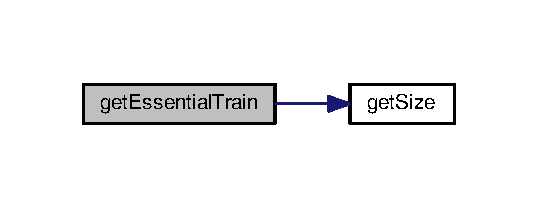
\includegraphics[width=258pt]{namespacetoolsBDD_ab85cfda40b715e400dda4a5e5c97f9ce_cgraph}
\end{center}
\end{figure}


\hypertarget{namespacetoolsBDD_ad9d092a50decbd07a5130e144731caa9}{\index{tools\-B\-D\-D@{tools\-B\-D\-D}!get\-Real@{get\-Real}}
\index{get\-Real@{get\-Real}!toolsBDD@{tools\-B\-D\-D}}
\subsubsection[{get\-Real}]{\setlength{\rightskip}{0pt plus 5cm}def tools\-B\-D\-D.\-get\-Real (
\begin{DoxyParamCaption}
\item[{}]{d, }
\item[{}]{si, }
\item[{}]{a}
\end{DoxyParamCaption}
)}}\label{namespacetoolsBDD_ad9d092a50decbd07a5130e144731caa9}


permet de contaner les realisateurs dans une chaine de char 


\begin{DoxyParams}{Paramètres}
{\em d} & toutes les lignes \\
\hline
{\em si} & nombre de lignes \\
\hline
{\em a} & le numero de la ligne courante \\
\hline
\end{DoxyParams}


Voici le graphe des appelants de cette fonction \-:\nopagebreak
\begin{figure}[H]
\begin{center}
\leavevmode
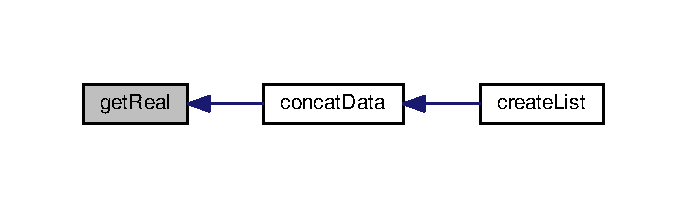
\includegraphics[width=330pt]{namespacetoolsBDD_ad9d092a50decbd07a5130e144731caa9_icgraph}
\end{center}
\end{figure}


\hypertarget{namespacetoolsBDD_ae224e914a0d4d23030401af6e59cb1bc}{\index{tools\-B\-D\-D@{tools\-B\-D\-D}!get\-Size@{get\-Size}}
\index{get\-Size@{get\-Size}!toolsBDD@{tools\-B\-D\-D}}
\subsubsection[{get\-Size}]{\setlength{\rightskip}{0pt plus 5cm}def tools\-B\-D\-D.\-get\-Size (
\begin{DoxyParamCaption}
\item[{}]{a}
\end{DoxyParamCaption}
)}}\label{namespacetoolsBDD_ae224e914a0d4d23030401af6e59cb1bc}


permet de savoir le nombre de hits 


\begin{DoxyParams}{Paramètres}
{\em a} & les lignes de la base \\
\hline
\end{DoxyParams}
\begin{DoxyReturn}{Renvoie}
le nombre de ligne 
\end{DoxyReturn}


Voici le graphe des appelants de cette fonction \-:\nopagebreak
\begin{figure}[H]
\begin{center}
\leavevmode
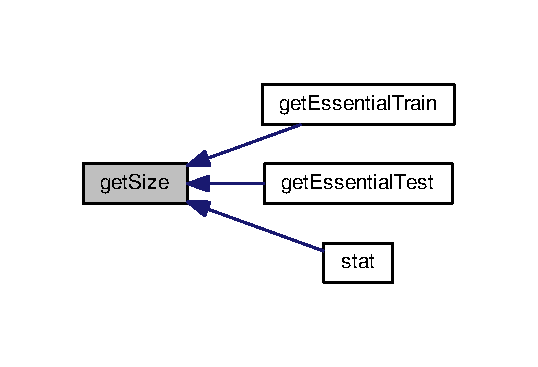
\includegraphics[width=258pt]{namespacetoolsBDD_ae224e914a0d4d23030401af6e59cb1bc_icgraph}
\end{center}
\end{figure}


\hypertarget{namespacetoolsBDD_a49928e1495cbb0687a8656f3c5481d5b}{\index{tools\-B\-D\-D@{tools\-B\-D\-D}!get\-Test@{get\-Test}}
\index{get\-Test@{get\-Test}!toolsBDD@{tools\-B\-D\-D}}
\subsubsection[{get\-Test}]{\setlength{\rightskip}{0pt plus 5cm}def tools\-B\-D\-D.\-get\-Test (
\begin{DoxyParamCaption}
\item[{}]{dic, }
\item[{}]{s}
\end{DoxyParamCaption}
)}}\label{namespacetoolsBDD_a49928e1495cbb0687a8656f3c5481d5b}


return an index for tfidf, None if doesn't exist 


\begin{DoxyParams}{Paramètres}
{\em dict} & dictionnaire \\
\hline
{\em s} & nom du labels \\
\hline
\end{DoxyParams}
\begin{DoxyReturn}{Renvoie}
valeur pour ce label 
\end{DoxyReturn}
\hypertarget{namespacetoolsBDD_ae5e38adc6d6db8e1ece60d2bc307a39f}{\index{tools\-B\-D\-D@{tools\-B\-D\-D}!init@{init}}
\index{init@{init}!toolsBDD@{tools\-B\-D\-D}}
\subsubsection[{init}]{\setlength{\rightskip}{0pt plus 5cm}def tools\-B\-D\-D.\-init (
\begin{DoxyParamCaption}
{}
\end{DoxyParamCaption}
)}}\label{namespacetoolsBDD_ae5e38adc6d6db8e1ece60d2bc307a39f}


permet de charger dans la base de donnee 

\hypertarget{namespacetoolsBDD_a82b711337498f7fa58e3c9d784415424}{\index{tools\-B\-D\-D@{tools\-B\-D\-D}!ranking@{ranking}}
\index{ranking@{ranking}!toolsBDD@{tools\-B\-D\-D}}
\subsubsection[{ranking}]{\setlength{\rightskip}{0pt plus 5cm}def tools\-B\-D\-D.\-ranking (
\begin{DoxyParamCaption}
\item[{}]{t, }
\item[{}]{x}
\end{DoxyParamCaption}
)}}\label{namespacetoolsBDD_a82b711337498f7fa58e3c9d784415424}


calcul le nombre de film dont le score $>$= x 


\begin{DoxyParams}{Paramètres}
{\em t} & une ligne \\
\hline
{\em x} & number de comparaison \\
\hline
\end{DoxyParams}
\begin{DoxyReturn}{Renvoie}
le nombre 
\end{DoxyReturn}


Voici le graphe des appelants de cette fonction \-:\nopagebreak
\begin{figure}[H]
\begin{center}
\leavevmode
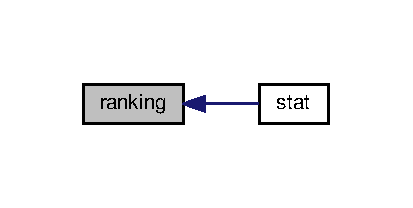
\includegraphics[width=198pt]{namespacetoolsBDD_a82b711337498f7fa58e3c9d784415424_icgraph}
\end{center}
\end{figure}


\hypertarget{namespacetoolsBDD_a2e502b4dae284eb951de46e92134895f}{\index{tools\-B\-D\-D@{tools\-B\-D\-D}!stat@{stat}}
\index{stat@{stat}!toolsBDD@{tools\-B\-D\-D}}
\subsubsection[{stat}]{\setlength{\rightskip}{0pt plus 5cm}def tools\-B\-D\-D.\-stat (
\begin{DoxyParamCaption}
\item[{}]{a}
\end{DoxyParamCaption}
)}}\label{namespacetoolsBDD_a2e502b4dae284eb951de46e92134895f}


permet de calculer et d'afficher des statistiques 


\begin{DoxyParams}{Paramètres}
{\em a} & liste de lignes \\
\hline
\end{DoxyParams}
\begin{DoxyReturn}{Renvoie}
moyenne et autres stats 
\end{DoxyReturn}


Voici le graphe d'appel pour cette fonction \-:\nopagebreak
\begin{figure}[H]
\begin{center}
\leavevmode
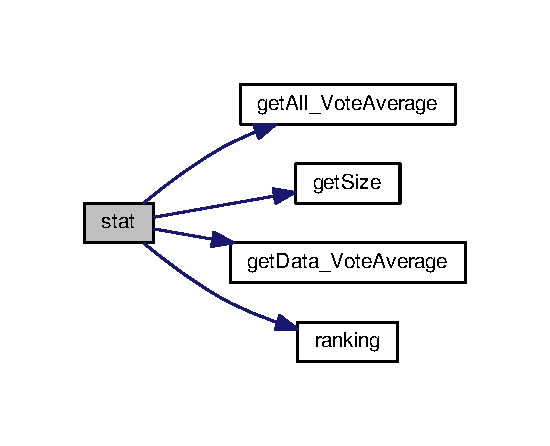
\includegraphics[width=264pt]{namespacetoolsBDD_a2e502b4dae284eb951de46e92134895f_cgraph}
\end{center}
\end{figure}


\hypertarget{namespacetoolsBDD_a73bb9d4526a9cd6825636ef1a5777106}{\index{tools\-B\-D\-D@{tools\-B\-D\-D}!test\-\_\-success@{test\-\_\-success}}
\index{test\-\_\-success@{test\-\_\-success}!toolsBDD@{tools\-B\-D\-D}}
\subsubsection[{test\-\_\-success}]{\setlength{\rightskip}{0pt plus 5cm}def tools\-B\-D\-D.\-test\-\_\-success (
\begin{DoxyParamCaption}
\item[{}]{X, }
\item[{}]{Y, }
\item[{}]{index}
\end{DoxyParamCaption}
)}}\label{namespacetoolsBDD_a73bb9d4526a9cd6825636ef1a5777106}


permet de savoir si cela est un succes 


\begin{DoxyParams}{Paramètres}
{\em X} & resultat de la tfidf \\
\hline
{\em y} & vecteur de la tfidf  predicat \\
\hline
\end{DoxyParams}
\begin{DoxyReturn}{Renvoie}
if t $<$ 0 -\/$>$ success else clear 
\end{DoxyReturn}
\hypertarget{namespacetoolsBDD_a07b4809d77a061cf4c10d05b35edf657}{\index{tools\-B\-D\-D@{tools\-B\-D\-D}!test\-\_\-success2@{test\-\_\-success2}}
\index{test\-\_\-success2@{test\-\_\-success2}!toolsBDD@{tools\-B\-D\-D}}
\subsubsection[{test\-\_\-success2}]{\setlength{\rightskip}{0pt plus 5cm}def tools\-B\-D\-D.\-test\-\_\-success2 (
\begin{DoxyParamCaption}
\item[{}]{X, }
\item[{}]{Y, }
\item[{}]{index}
\end{DoxyParamCaption}
)}}\label{namespacetoolsBDD_a07b4809d77a061cf4c10d05b35edf657}


permet de savoir si cela est un succes 


\begin{DoxyParams}{Paramètres}
{\em X} & resultat de la tfidf \\
\hline
{\em y} & vecteur de la tfidf  predicat \\
\hline
\end{DoxyParams}
\begin{DoxyReturn}{Renvoie}
if t $<$ 0 -\/$>$ success else clear 
\end{DoxyReturn}
\hypertarget{namespacetoolsBDD_accbe8232ffba571517272bcd0eb22df7}{\index{tools\-B\-D\-D@{tools\-B\-D\-D}!transform@{transform}}
\index{transform@{transform}!toolsBDD@{tools\-B\-D\-D}}
\subsubsection[{transform}]{\setlength{\rightskip}{0pt plus 5cm}def tools\-B\-D\-D.\-transform (
\begin{DoxyParamCaption}
\item[{}]{pairs, }
\item[{}]{vocabulary = {\ttfamily None}}
\end{DoxyParamCaption}
)}}\label{namespacetoolsBDD_accbe8232ffba571517272bcd0eb22df7}


permet d'effectuer un tfidf 


\begin{DoxyParams}{Paramètres}
{\em pairs} & le texte \\
\hline
{\em vocabulary} & vocabulaire sur lequel applique l'algorithme \\
\hline
\end{DoxyParams}
\begin{DoxyReturn}{Renvoie}
tf-\/idf + vector 
\end{DoxyReturn}

\chapter{Documentation des classes}
\hypertarget{classBDD_1_1BDD}{\section{Référence de la classe B\-D\-D}
\label{classBDD_1_1BDD}\index{B\-D\-D@{B\-D\-D}}
}


Graphe de collaboration de B\-D\-D\-:\nopagebreak
\begin{figure}[H]
\begin{center}
\leavevmode
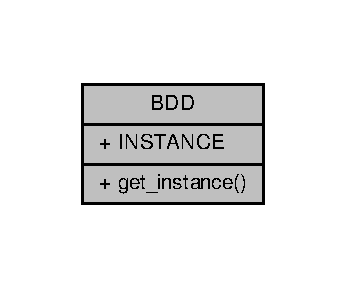
\includegraphics[width=166pt]{classBDD_1_1BDD__coll__graph}
\end{center}
\end{figure}
\subsection*{Fonctions membres publiques}
\begin{DoxyCompactItemize}
\item 
def \hyperlink{classBDD_1_1BDD_a36acd77a41a08a7a2ce682c5336801e0}{get\-\_\-instance}
\end{DoxyCompactItemize}
\subsection*{Attributs publics statiques}
\begin{DoxyCompactItemize}
\item 
\hyperlink{classBDD_1_1BDD_acdc4eb469ce81b047ec0acf8bfaa6e22}{I\-N\-S\-T\-A\-N\-C\-E} = None
\end{DoxyCompactItemize}


\subsection{Documentation des fonctions membres}
\hypertarget{classBDD_1_1BDD_a36acd77a41a08a7a2ce682c5336801e0}{\index{B\-D\-D\-::\-B\-D\-D@{B\-D\-D\-::\-B\-D\-D}!get\-\_\-instance@{get\-\_\-instance}}
\index{get\-\_\-instance@{get\-\_\-instance}!BDD::BDD@{B\-D\-D\-::\-B\-D\-D}}
\subsubsection[{get\-\_\-instance}]{\setlength{\rightskip}{0pt plus 5cm}def get\-\_\-instance (
\begin{DoxyParamCaption}
\item[{}]{cls}
\end{DoxyParamCaption}
)}}\label{classBDD_1_1BDD_a36acd77a41a08a7a2ce682c5336801e0}


\subsection{Documentation des données membres}
\hypertarget{classBDD_1_1BDD_acdc4eb469ce81b047ec0acf8bfaa6e22}{\index{B\-D\-D\-::\-B\-D\-D@{B\-D\-D\-::\-B\-D\-D}!I\-N\-S\-T\-A\-N\-C\-E@{I\-N\-S\-T\-A\-N\-C\-E}}
\index{I\-N\-S\-T\-A\-N\-C\-E@{I\-N\-S\-T\-A\-N\-C\-E}!BDD::BDD@{B\-D\-D\-::\-B\-D\-D}}
\subsubsection[{I\-N\-S\-T\-A\-N\-C\-E}]{\setlength{\rightskip}{0pt plus 5cm}I\-N\-S\-T\-A\-N\-C\-E = None\hspace{0.3cm}{\ttfamily [static]}}}\label{classBDD_1_1BDD_acdc4eb469ce81b047ec0acf8bfaa6e22}


La documentation de cette classe a été générée à partir du fichier suivant \-:\begin{DoxyCompactItemize}
\item 
\hyperlink{BDD_8py}{B\-D\-D.\-py}\end{DoxyCompactItemize}

\chapter{Documentation des fichiers}
\hypertarget{algo_8py}{\section{Référence du fichier algo.\-py}
\label{algo_8py}\index{algo.\-py@{algo.\-py}}
}
\subsection*{Espaces de nommage}
\begin{DoxyCompactItemize}
\item 
\hyperlink{namespacealgo}{algo}
\end{DoxyCompactItemize}
\subsection*{Fonctions}
\begin{DoxyCompactItemize}
\item 
def \hyperlink{namespacealgo_a802d43423d0ac8fd6a52cc2508186072}{accuraccy\-\_\-test}
\begin{DoxyCompactList}\small\item\em permet de savoir si c'est un echec ou succes \end{DoxyCompactList}\item 
def \hyperlink{namespacealgo_ab46541a846c7f71c15e9bae5d5836af7}{algo\-Tree}
\begin{DoxyCompactList}\small\item\em permet de lancer pour les deux arbres \end{DoxyCompactList}\item 
def \hyperlink{namespacealgo_a70c4b2737389dbfb07be3b39a8cf8e9b}{find\-\_\-best\-\_\-k\-\_\-for\-\_\-kneighbors}
\begin{DoxyCompactList}\small\item\em permet de savoir le meilleur k possible \end{DoxyCompactList}\item 
def \hyperlink{namespacealgo_a4227080ec2328a03c4f6f01e7b022e08}{generic\-\_\-tree}
\begin{DoxyCompactList}\small\item\em permet de savoir les meilleurs parametres \end{DoxyCompactList}\item 
def \hyperlink{namespacealgo_a0afe8d007fc92279c75be5d0b40ecf07}{generic\-\_\-tree\-\_\-score}
\begin{DoxyCompactList}\small\item\em permet de savoir si c'est un echec ou succes \end{DoxyCompactList}\item 
def \hyperlink{namespacealgo_a5ecd48a13b42118beac0652265b8f353}{naive\-Bayes}
\begin{DoxyCompactList}\small\item\em permet de savoir si c'est un echec ou succes \end{DoxyCompactList}\end{DoxyCompactItemize}

\hypertarget{BDD_8py}{\section{Référence du fichier B\-D\-D.\-py}
\label{BDD_8py}\index{B\-D\-D.\-py@{B\-D\-D.\-py}}
}
\subsection*{Classes}
\begin{DoxyCompactItemize}
\item 
class \hyperlink{classBDD_1_1BDD}{B\-D\-D}
\end{DoxyCompactItemize}
\subsection*{Espaces de nommage}
\begin{DoxyCompactItemize}
\item 
\hyperlink{namespaceBDD}{B\-D\-D}
\end{DoxyCompactItemize}
\subsection*{Variables}
\begin{DoxyCompactItemize}
\item 
string \hyperlink{namespaceBDD_a5b93a013f8d46f91f8d7b0fc102a42e7}{index} = \char`\"{}fouille\char`\"{}
\item 
string \hyperlink{namespaceBDD_ab065e06b98ff8f50dcdabe5715c5b710}{table\-Credit\-Test} = \char`\"{}Test\-Credit\char`\"{}
\item 
string \hyperlink{namespaceBDD_a5453a62b7989a6ea0d9d1f4016411323}{table\-Credit\-Train} = \char`\"{}Train\-Credit\char`\"{}
\item 
string \hyperlink{namespaceBDD_a1a3347461ee00b8dba8e995423d6acea}{table\-Movie\-Test} = \char`\"{}Test\-Movie\char`\"{}
\item 
string \hyperlink{namespaceBDD_a69bea8ff9373a0baf5bbf3df09f7a3b0}{table\-Movie\-Train} = \char`\"{}Train\-Movie\char`\"{}
\end{DoxyCompactItemize}

\hypertarget{main_8py}{\section{Référence du fichier main.\-py}
\label{main_8py}\index{main.\-py@{main.\-py}}
}
\subsection*{Espaces de nommage}
\begin{DoxyCompactItemize}
\item 
\hyperlink{namespacemain}{main}
\end{DoxyCompactItemize}
\subsection*{Variables}
\begin{DoxyCompactItemize}
\item 
tuple \hyperlink{namespacemain_a3ba02571b750dd172f300851ef10228e}{dic} = to.\-get\-Dict(tfidf)
\item 
tuple \hyperlink{namespacemain_abc599b1f87ca3a4e0ff709091fb25176}{l} = to.\-create\-List(d, s)
\item 
tuple \hyperlink{namespacemain_a2187ed276d33f5f18ef29ecf5ce613ba}{lt} = to.\-create\-List(dt, st)
\item 
tuple \hyperlink{namespacemain_a7a74e6f2f6355f34b63513f77c839a9e}{x} = al.\-find\-\_\-best\-\_\-k\-\_\-for\-\_\-kneighbors(mat, vec)
\end{DoxyCompactItemize}

\hypertarget{operatorBDD_8py}{\section{Référence du fichier operator\-B\-D\-D.\-py}
\label{operatorBDD_8py}\index{operator\-B\-D\-D.\-py@{operator\-B\-D\-D.\-py}}
}
\subsection*{Espaces de nommage}
\begin{DoxyCompactItemize}
\item 
\hyperlink{namespaceoperatorBDD}{operator\-B\-D\-D}
\end{DoxyCompactItemize}
\subsection*{Fonctions}
\begin{DoxyCompactItemize}
\item 
def \hyperlink{namespaceoperatorBDD_a5aaccf3717ce1479bbd6ef2a0ffcbf49}{B\-D\-Dfrom\-C\-S\-V}
\begin{DoxyCompactList}\small\item\em permet de stocker dans elasticsearch les donnees dans fichiers \end{DoxyCompactList}\item 
def \hyperlink{namespaceoperatorBDD_a9890bc0308c65dae331300c93f804b11}{B\-D\-D\-Search}
\begin{DoxyCompactList}\small\item\em cherche dans la table, la requete et renvoi le resultat \end{DoxyCompactList}\item 
def \hyperlink{namespaceoperatorBDD_a84ebaeadd8b021780f5fa72f73bf3ea3}{B\-D\-D\-Search\-All}
\begin{DoxyCompactList}\small\item\em cherche dans la table train, tout les documents \end{DoxyCompactList}\item 
def \hyperlink{namespaceoperatorBDD_aa9ab222b23d1b7a6e094fb82d702cd0a}{B\-D\-D\-Search\-All\-Test}
\begin{DoxyCompactList}\small\item\em cherche dans la table test, tout les documents \end{DoxyCompactList}\item 
def \hyperlink{namespaceoperatorBDD_a03889cf9d5fd998892c621491a12142b}{B\-D\-D\-Search\-Categorie}
\begin{DoxyCompactList}\small\item\em cherche dans la table train, tout les documents ayant tel key et value \end{DoxyCompactList}\item 
def \hyperlink{namespaceoperatorBDD_a30969a6c243559357c836ae43365877b}{B\-D\-D\-Search\-Categorie\-Test}
\begin{DoxyCompactList}\small\item\em cherche dans la table test, tout les documents ayant tel key et value \end{DoxyCompactList}\end{DoxyCompactItemize}
\subsection*{Variables}
\begin{DoxyCompactItemize}
\item 
float \hyperlink{namespaceoperatorBDD_a131e5e7a22125521cf2cb5eb732a0f54}{mediane\-Vote\-Average} = 6.\-2
\end{DoxyCompactItemize}

\hypertarget{toolsBDD_8py}{\section{Référence du fichier tools\-B\-D\-D.\-py}
\label{toolsBDD_8py}\index{tools\-B\-D\-D.\-py@{tools\-B\-D\-D.\-py}}
}
\subsection*{Espaces de nommage}
\begin{DoxyCompactItemize}
\item 
\hyperlink{namespacetoolsBDD}{tools\-B\-D\-D}
\end{DoxyCompactItemize}
\subsection*{Fonctions}
\begin{DoxyCompactItemize}
\item 
def \hyperlink{namespacetoolsBDD_abf21310dd3cdd39ff5f781eaafb23b24}{concat\-Data}
\begin{DoxyCompactList}\small\item\em permet de concatener les valeurs \end{DoxyCompactList}\item 
def \hyperlink{namespacetoolsBDD_afc4367a1a711e612f8f4d6363edbc640}{create\-List}
\begin{DoxyCompactList}\small\item\em liste of tuple \end{DoxyCompactList}\item 
def \hyperlink{namespacetoolsBDD_a60efb6c205d51bf9a9e32b6d19f633b4}{get\-\_\-train\-\_\-test\-\_\-sets}
\begin{DoxyCompactList}\small\item\em permet de creer faire des separation pour la validation croisee \end{DoxyCompactList}\item 
def \hyperlink{namespacetoolsBDD_ae897b96e0c4a89d09f418e620819a066}{get\-All\-\_\-\-Vote\-Average}
\begin{DoxyCompactList}\small\item\em recuperer tous les votes \end{DoxyCompactList}\item 
def \hyperlink{namespacetoolsBDD_a15b2ef52eec23442bb79863d794e2e2b}{get\-Cast}
\begin{DoxyCompactList}\small\item\em permet de contaner les valeurs des 6 acteurs dans une chaine de char \end{DoxyCompactList}\item 
def \hyperlink{namespacetoolsBDD_ab6a097315bef68f12966b652fd120913}{get\-Data}
\begin{DoxyCompactList}\small\item\em permet de contaner les valeurs dans une chaine de char \end{DoxyCompactList}\item 
def \hyperlink{namespacetoolsBDD_a1815eb69cbba2e6abc16b649baa2fdad}{get\-Data\-\_\-\-Vote\-Average}
\begin{DoxyCompactList}\small\item\em calcul des statistiques sur le champ vote\-\_\-average \end{DoxyCompactList}\item 
def \hyperlink{namespacetoolsBDD_aef96b5903d59864e793f4377d82bac25}{get\-Dict}
\begin{DoxyCompactList}\small\item\em permet de connaitre les labels dune tfidf \end{DoxyCompactList}\item 
def \hyperlink{namespacetoolsBDD_abc6b8127dc8f28edc53d719a4835bfa3}{get\-Essential\-Test}
\begin{DoxyCompactList}\small\item\em permet de recuperer les infos pour ensemble de train \end{DoxyCompactList}\item 
def \hyperlink{namespacetoolsBDD_ab85cfda40b715e400dda4a5e5c97f9ce}{get\-Essential\-Train}
\begin{DoxyCompactList}\small\item\em permet de recuperer les infos pour ensemble de train \end{DoxyCompactList}\item 
def \hyperlink{namespacetoolsBDD_ad9d092a50decbd07a5130e144731caa9}{get\-Real}
\begin{DoxyCompactList}\small\item\em permet de contaner les realisateurs dans une chaine de char \end{DoxyCompactList}\item 
def \hyperlink{namespacetoolsBDD_ae224e914a0d4d23030401af6e59cb1bc}{get\-Size}
\begin{DoxyCompactList}\small\item\em permet de savoir le nombre de hits \end{DoxyCompactList}\item 
def \hyperlink{namespacetoolsBDD_a49928e1495cbb0687a8656f3c5481d5b}{get\-Test}
\begin{DoxyCompactList}\small\item\em return an index for tfidf, None if doesn't exist \end{DoxyCompactList}\item 
def \hyperlink{namespacetoolsBDD_ae5e38adc6d6db8e1ece60d2bc307a39f}{init}
\begin{DoxyCompactList}\small\item\em permet de charger dans la base de donnee \end{DoxyCompactList}\item 
def \hyperlink{namespacetoolsBDD_a82b711337498f7fa58e3c9d784415424}{ranking}
\begin{DoxyCompactList}\small\item\em calcul le nombre de film dont le score $>$= x \end{DoxyCompactList}\item 
def \hyperlink{namespacetoolsBDD_a2e502b4dae284eb951de46e92134895f}{stat}
\begin{DoxyCompactList}\small\item\em permet de calculer et d'afficher des statistiques \end{DoxyCompactList}\item 
def \hyperlink{namespacetoolsBDD_a73bb9d4526a9cd6825636ef1a5777106}{test\-\_\-success}
\begin{DoxyCompactList}\small\item\em permet de savoir si cela est un succes \end{DoxyCompactList}\item 
def \hyperlink{namespacetoolsBDD_accbe8232ffba571517272bcd0eb22df7}{transform}
\begin{DoxyCompactList}\small\item\em permet d'effectuer un tfidf \end{DoxyCompactList}\end{DoxyCompactItemize}

%--- End generated contents ---

% Index
\newpage
\phantomsection
\addcontentsline{toc}{chapter}{Index}
\printindex

\end{document}
